
\chapter{Přehled převzaté práce}
\label{prevzanaPrace}

V této příloze je uveden rozpis jednotlivých modulů výsledného softwaru a míra, do které jsem k implementaci modulu přispěl.

\begin{table}[h]
\centering
\begin{tabular}{|l|c|c|c|c|}
\hline
Modul                      & Původní & Refaktorizován & Nový \\ \hline
\hline
Rozhraní procesoru         &         &                & \checkmark     \\ \hline
Registry a registrové pole &         &                & \checkmark     \\ \hline
Fáze Fetch, Decode         &         & \checkmark     &      \\ \hline
ROB                        &         & \checkmark     &      \\ \hline
Předpověď skoků            &         & \checkmark     &      \\ \hline
Fáze Execute               &         & \checkmark     &      \\ \hline
Reprezentace instrukcí     &         & \checkmark     &      \\ \hline
Interpretace instrukcí     &         &                & \checkmark     \\ \hline
Paměti a cache             &         & \checkmark     &      \\ \hline
Alokace polí v paměti      &         &                & \checkmark    \\ \hline
Parsování a překlad kódu   &         &                & \checkmark    \\ \hline
Nastavení simulace         &         & \checkmark     &      \\ \hline
Sběr statistik             &         & \checkmark     &      \\ \hline
Server, serializace        &         &                & \checkmark    \\ \hline
Instrukční sada RISC-V     &         & \checkmark     &      \\ \hline % todo nešel sem dát footnote (doplnění nových instrukcí
Testy                      &         & \checkmark     &      \\ \hline
Webové rozhraní            &         &                & \checkmark    \\ \hline
Rozhraní příkazové řádky   &         &                & \checkmark    \\ \hline
Kontejnerizace             &         &                & \checkmark    \\ \hline
Příklady programů a konfigurace &         & \checkmark     &      \\ \hline
\end{tabular}
\caption{Přehled modulů a můj přínos implementaci.}
\label{myworkTable}
\end{table}

\chapter{Statistiky sbírané při simulaci}
\label{statsAppend}

V této příloze je uvedena tabulka jednotlivých metrik sbíraných v rámci simulace činnosti procesoru.
Použité datové typy jsou z jazyka Java.
Statistiky jsou konzumovány ve formátu JSON, kde tyto datové typy mají svůj ekvivalent.

\begin{table}[!ht]
    \centering
    \begin{tabular}{|l|l|p{6cm}|}
    \hline
        Statistika & Datový typ & Popis pole \\ \hline\hline
        staticInstructionMix & InstructionMix & Uchovává statický instrukční mix \\ 
        dynamicInstructionMix & InstructionMix & Uchovává dynamický instrukční mix \\ 
        cache & CacheStatistics & Statistiky cache \\ 
        fuStats & Map<String, FUStats> & Statistiky funkčních jednotek \\ 
        instructionStats & List<InstructionStats> & Statistiky pro každou instrukci \\ 
        committedInstructions & long & Počet vydaných instrukcí \\ 
        clockCycles & long & Počet taktů výpočtu \\ 
        flushedInstructions & long & Počet zahozených instrukcí z důvodu špatné predikce skoku \\ 
        robFlushes & long & Počet vypláchnutí ROB \\ 
        clock & int & Frekvence hodin (Hz) \\ 
        correctlyPredictedBranches & long & Počet správně předpovězených skoků \\ 
        conditionalBranches & long & Počet podmíněných skoků \\ 
        takenBranches & long & Počet provedených skoků \\ 
        mainMemoryLoadedBytes & long & Množství dat přenesených z hlavní paměti \\ 
        mainMemoryStoredBytes & long & Množství dat přenesených do hlavní paměti \\ 
        maxAllocatedRegisters & int & Maximální počet přidělených spekulativních registrů \\ \hline
    \end{tabular}
    \caption{Hlavní objekt statistiky.}
    \label{mainstatsTable}
\end{table}

\begin{table}[!ht]
    \centering
    \begin{tabular}{|l|l|l|}
    \hline
        Statistika & Datový typ & Popis pole \\ \hline\hline
        intArithmetic & int & Počet celočíselných aritmetických operací \\ 
        floatArithmetic & int & Počet operací s pohyblivou desetinnou čárkou \\ 
        memory & int & Počet paměťových operací \\ 
        branch & int & Počet instrukcí skoku \\ 
        other & int & Počet ostatních instrukcí \\ \hline
    \end{tabular}
    \caption{Objekt pro popis statického nebo dynamického instrukčního mixu.}
    \label{InstructionMixTable}
\end{table}

\begin{table}[!ht]
    \centering
    \begin{tabular}{|l|l|l|}
    \hline
        Statistika & Datový typ & Popis pole \\ \hline\hline
        readAccesses & int & Počet čtení z cache \\ 
        writeAccesses & int & Počet zápisů do cache \\ 
        hits & int & Počet úspěšných přístupů do cache \\ 
        misses & int & Počet neúspěšných přístupů do cache \\ 
        totalDelay & int & Celkové zpoždění způsobené přístupy do cache \\ 
        bytesWritten & int & Počet bytů zapsaných do cache \\ 
        bytesRead & int & Počet přečtených bytů z cache \\ \hline
    \end{tabular}
    \caption{Statistiky týkající se cache.}
    \label{CacheStatisticsTable}
\end{table}

\chapter{Argumenty simulátoru}
\label{simArgs}

Níže jsou uvedeny argumenty příkazové řádky pro simulátor.
Argumenty jsou rozděleny do dvou skupin: argumenty pro spouštění v příkazové řádce (tabulka \ref{cliArgsTable}) a argumenty pro spouštění serveru (tabulka \ref{serverArgsTable}).

Spuštění programu se skládá z názvu programu, režimu (\texttt{cli} nebo \texttt{server}) a argumentů.
Příklady spuštění jsou uvedeny v kódu \ref{runshExample}.
Příklady jsou v ukázce spouštěny ze složky \texttt{Sources/simulator}.
V případě jiného způsobu instalace je nutné nahradit \texttt{./scripts/run.sh} jinou cestou.

\begin{figure}[hbtp]
\begin{lstlisting}[]
./scripts/run.sh cli \
  --cpu examples/cpuConfigurations/default.json \
  --program examples/asmPrograms/basicLoadStore.r5
# nebo
./scripts/run.sh server
\end{lstlisting}
\caption{Příklad spuštění simulátoru v režimech cli a server.}
\label{runshExample}
\end{figure}

\begin{table}[!ht]
    \centering
    \begin{tabular}{|l|l|l|}
    \hline
        Argument & Povinný & Popis \\ \hline\hline
        \texttt{--entry=LABEL|ADDRESS} & Ne & Adresa nebo návěští počátku programu. \\ 
        \texttt{--pretty} & Ne & Formátování JSON výstupu. \\ 
        \texttt{--full-state} & Ne & Plný výstup. Ve výchozím režimu je výstup zkrácený. \\
        \texttt{--cpu=<soubor>} & Ano & Konfigurace procesoru. \\ 
        \texttt{--program=<soubor>} & Ano & Program v assembleru RISC-V. \\ 
        \texttt{--memory=<soubor>} & Ne & Konfigurace paměti. \\ \hline
    \end{tabular}
    \caption{Argumenty příkazu \texttt{cli}, který spouští simulaci z příkazové řádky. Argumenty s parametrem \texttt{<soubor>} očekávají cestu k souboru.}
    \label{cliArgsTable}
\end{table}

\begin{table}[!ht]
    \centering
    \begin{tabular}{|l|l|l|p{6cm}|}
    \hline
        Argument & Povinný & Výchozí hodnota & Popis \\ \hline\hline
        \texttt{--gcc-path=PATH} & Ne & -- & Cesta k překladači GCC \\
        \texttt{--host=ADDR} & Ne & 0.0.0.0 & Adresa, ke které se má server připojit \\
        \texttt{--port=PORT} & Ne & 8\,000  & Port, ke kterému se má server připojit \\
        \texttt{--timeout-ms=NUMBER} & Ne & 30\,000 & Časový limit pro požadavky v milisekundách \\ \hline
    \end{tabular}
    \caption{Argumenty příkazu \texttt{server}, který spouští HTTP server.}
    \label{serverArgsTable}
\end{table}


\chapter{Konfigurace procesoru}
\label{cpuConfigAppendice}

Následující tabulky popisují parametry procesoru.
Tyto parametry jsou přijímány při požadavku na simulaci jak v CLI tak HTTP režimu simulátoru.
Konkrétní příklady konfigurací ve formátu JSON jsou k nalezení v přiloženém kódu.

\subsection*{Tabulka 1: Konfigurace bufferu}

\begin{tabular}{|l|l|l|p{7cm}|}
\hline
Parametr & Typ & Přijatelné hodnoty & Popis \\
\hline
\texttt{robSize} & int & 1 až 1024 & Maximální počet instrukcí, které mohou být v ROB. \\
\texttt{commitWidth} & int & 1 až 10 & Počet instrukcí, které mohou být potvrzeny během jednoho cyklu - commitLimit v ROB. \\
\texttt{flushPenalty} & int & 0 až 100 & Počet cyklů hodin, které CPU potřebuje k vyprázdnění pipeline. \\
\texttt{fetchWidth} & int & 1 až 10 & Počet instrukcí, které lze načíst během jednoho cyklu. \\
\hline
\end{tabular}

\subsection*{Tabulka 2: Konfigurace predikce}

\begin{tabular}{|l|l|p{5.6cm}|p{3cm}|}
\hline
Parametr & Typ & Přijatelné hodnoty & Popis \\
\hline
\texttt{useGlobalHistory} & boolean & true nebo false & Použití globální historie ve vektoru PHT. \\
\texttt{btbSize} & int & 1 až 16384 & Velikost bufferu cílů větve. \\
\texttt{phtSize} & int & 1 až 16384 & Velikost tabulky historie vzoru. \\
\texttt{predictorType} & String & "ZERO\_BIT\_PREDICTOR", "ONE\_BIT\_PREDICTOR", "TWO\_BIT\_PREDICTOR" & Typ prediktoru uloženého v PHT. \\
\texttt{predictorDefault} & int & Pro "ZERO\_BIT\_PREDICTOR": 0, 1. Pro "ONE\_BIT\_PREDICTOR": 0 až 3. Pro "TWO\_BIT\_PREDICTOR": 0 až 3. & Počáteční stav všech prediktorů. \\
\hline
\end{tabular}

\subsection*{Tabulka 3: Konfigurace funkčních jednotek}

\begin{tabular}{|l|p{4.1cm}|p{3.5cm}|p{4cm}|}
\hline
Parametr & Typ & Přijatelné hodnoty & Popis \\
\hline
\texttt{fUnits} & Pole popisu \texttt{Functional\-Unit\-Description} & Not null, Not empty & Seznam jednotek FU nesmí být null a musí obsahovat alespoň jednu jednotku FU. \\
\hline
\end{tabular}

\subsection*{Tabulka 4: Konfigurace funkční jednotky FX/FP\footnote{Jedná se o třídu \texttt{Functional\-Unit\-Description}}}

\begin{tabular}{|l|l|l|p{4.95cm}|}
\hline
Parametr & Typ & Přijatelné hodnoty & Popis \\
\hline
\texttt{fuType} & Výčet (FX, FP) & FX nebo FP & Typ funkční jednotky (FX nebo FP). \\
\texttt{operations} & Pole \texttt{Capability} & Viz Tabulka X & Seznam schopností pro jednotky FX/FP. \\
\texttt{latency} & int & Nezáporná celá čísla & Latence zálohy (používá se pro typové převody). \\
\hline
\end{tabular}

\subsection*{Tabulka 5: Parametr \texttt{Capability}}

\begin{tabular}{|l|l|p{4.9cm}|p{4.8cm}|}
\hline
Parametr & Typ & Přijatelné hodnoty & Popis \\
\hline
\texttt{name} & \texttt{Capability} & addition, bitwise, multiplication, division, special & Název schopností pro jednotky FX/FP. \\
\texttt{latency} & int & Nezáporná celá čísla & Latence pro danou schopnost. \\
\hline
\end{tabular}

\subsection*{Tabulka 6: Konfigurace funkčních jednotek L\_S, Branch, Memory\footnote{Jedná se o třídu \texttt{Functional\-Unit\-Description}}}

\begin{tabular}{|l|p{3.5cm}|p{4cm}|p{5cm}|}
\hline
Parametr & Typ & Přijatelné hodnoty & Popis \\
\hline
\texttt{fuType} & Výčet (L\_S, Branch, Memory) & L\_S, Branch, nebo Memory & Typ funkční jednotky. \\
\texttt{latency} & int & Nezáporná celá čísla & Latence pro funkční jednotku. \\
\hline
\end{tabular}

\subsection*{Tabulka 7: Konfigurační parametry pro mezipaměť CPU}

\begin{tabular}{|l|l|p{4.2cm}|p{4.5cm}|}
\hline
Parametr & Typ & Přijatelné hodnoty & Popis \\
\hline
\texttt{useCache} & boolean & true, false & Povolit nebo zakázat mezipaměť jedné úrovně. \\
\texttt{cacheLines} & int & 1 až 65536 & Počet cache linek. \\
\texttt{cacheLineSize} & int & mocnina čísla 2 mezi 1 a 512 & Velikost jedné cache linky v bytech (musí být mocninou čísla 2). \\
\texttt{cacheAssoc} & int & 1 nebo více* & Asociativita cache (1 pro přímý mapovaný). \\
\texttt{cacheReplacement} & String & "Random", "LRU", "FIFO" & Politika nahrazení cache. \\
\texttt{storeBehavior} & String & "write-back", "write-through" & Politika zápisu do cache. \\
\texttt{laneReplacementDelay} & int & Nezáporné celé číslo & Cykly pro nahrazení cache linky. \\
\texttt{cacheAccessDelay} & int & Nezáporné celé číslo & Zpoždění přístupu do cache v cyklech. \\
\hline
\end{tabular}

\subsection*{Tabulka 8: Konfigurační parametry pro paměť CPU}

\begin{tabular}{|l|l|l|p{5.9cm}|}
\hline
Parametr & Typ & Přijatelné hodnoty & Popis \\
\hline
\texttt{lbSize} & int & 1 až 1024 & Velikost zásobníku pro načítání. \\
\texttt{sbSize} & int & 1 až 1024 & Velikost zásobníku pro ukládání. \\
\texttt{storeLatency} & int & Nezáporné celé číslo & Latence hlavní paměti pro operace ukládání. \\
\texttt{loadLatency} & int & Nezáporné celé číslo & Latence hlavní paměti pro operace načítání. \\
\texttt{callStackSize} & int & 0 až 65536 & Velikost zásobníku volání v bytech. \\
\texttt{speculativeRegisters} & int & 1 až 1024 & Počet spekulativních registrů. \\
\hline
\end{tabular}

\subsection*{Tabulka 9: Konfigurační parametry pro hodiny CPU}

\begin{tabular}{|l|l|l|p{6.4cm}|}
\hline
Parametr & Typ & Přijatelné hodnoty & Popis \\
\hline
\texttt{coreClockFrequency} & int & kladné celé číslo & Frekvence jádra procesoru v Hz. \\
\texttt{cacheClockFrequency} & int & kladné celé číslo & Frekvence mezipaměti procesoru v Hz. \\
\hline
\end{tabular}

\chapter{Pokyny pro spuštění aplikace}
\label{installSteps}

Tato příloha obsahuje pokyny ke spuštění kontejnerů Docker a manuální instalaci aplikace.

\section{Spuštění kontejnerů Docker}

Doporučeným a nejjednodušším způsobem provozu aplikace je pomocí připravených skriptů pro Docker (viz výpisy \ref{runContainer} a \ref{stopContainer}).
Jediným požadavkem je zde Docker, \texttt{docker compose} a internetové připojení.


\begin{lstlisting}[caption={Vytvoření a spuštění celé aplikace.},label=runContainer]
cd Sources && ./build_container.sh && ./run_container.sh
\end{lstlisting}

\begin{lstlisting}[caption={Zastavení obou kontejnerů.},label=stopContainer]
./stop_container.sh
\end{lstlisting}

\section{Manuální instalace}

Pro detailní instrukce k manuální instalaci nahlédněte do souborů \texttt{Sources/Readme.md} přiložených v médiu.

Požadavky pro provoz aplikace:
\begin{itemize}
    \item Java verze 17,
    \item npm verze 10.2.3,
    \item Node.js verze 21.2.0,
    \item GCC verze 12.3.0 pro RISC-V (pouze pro simulátor v režimu serveru).
\end{itemize}

Instrukce pro instalaci jsou uvedeny ve výpisu \ref{installSimulator}, příklad spuštění ve výpisu \ref{runCliSimulator}.

\begin{lstlisting}[caption={Posloupnost příkazů k instalaci a spuštění simulátoru.},label=installSimulator]
cd Sources/simulator
./scripts/install.sh
./scripts/run.sh help
\end{lstlisting}

\begin{lstlisting}[caption={Příklad supštění simulace v režimu CLI.},label=runCliSimulator]
./scripts/run.sh cli --cpu=examples/cpuConfigurations/default.json --program=examples/asmPrograms/basicFloatArithmetic.r5 --pretty
\end{lstlisting}


\chapter{Struktura zdrojových souborů}
\label{sourcemap}

Soubory přiložené v médiu obsahují projekty, zdrojový kód obou aplikací a kontejnerizační skripty (složka \texttt{Sources}) a dokumentaci (\texttt{Readme.md}, \texttt{Sources/frontend/Readme.md} a \texttt{Sources/simulator/Readme.md}).

% TODO přidat thesis a latex soubory sem i do repa

\dirtree{%
  .1 .
  .2 Readme.md.
  .2 .gitlab-ci.yml.
  .2 .gitlab.
  .2 Literature.
  .3 Web\_Based\_Simulator\_Of\_Superscalar\_Processors.pdf.
  .2 Thesis.
  .2 Sources.
  .3 docker-compose.yml.
  .3 build\_container.sh.
  .3 stop\_container.sh.
  .3 run\_container.sh.
  .3 frontend.
  .4 tailwind.config.ts.
  .4 package-lock.json.
  .4 Dockerfile.
  .4 .env.example.
  .4 tsconfig.json.
  .4 Readme.md.
  .4 biome.json.
  .4 package.json.
  .4 next-env.d.ts.
  .4 .gitignore.
  .4 next.config.mjs.
  .4 public.
  .4 src.
  .5 app.
  .6 \dots.
  .5 components.
  .6 \dots.
  .5 lib.
  .6 \dots.
  .5 \_\_tests\_\_.
  .6 \dots.
  .5 constant.
  .6 \dots.
  .5 styles.
  .6 \dots.
  .4 .swc.
  .5 plugins.
  .6 \dots.
  .3 test.
  .4 \dots.
  .3 simulator.
  .4 build.gradle.
  .4 Dockerfile.
  .4 Readme.md.
  .4 gradlew.
  .4 settings.gradle.
  .4 scripts.
  .5 install.sh.
  .5 run.sh.
  .5 runProd.sh.
  .5 testExamples.sh.
  .4 src.
  .5 test.
  .6 \dots.
  .5 jmh.
  .6 \dots.
  .5 main.
  .6 \dots.
  .4 examples.
  .5 simulations.
  .6 \dots.
  .5 cpuConfigurations.
  .6 \dots.
  .5 asmPrograms.
  .6 \dots.
  .5 memory.
  .6 \dots.
  .5 cPrograms.
  .6 \dots.
}\hfill

\chapter{Galerie webové aplikace}
\label{gallery}

% Obsahem této přílohy je několik snímků obrazovky z webového simulátoru.
% Obrázky začínají na následující straně.
\hspace{2.5cm}
\rotatebox{90}{\begin{minipage}{0.75\textheight}
    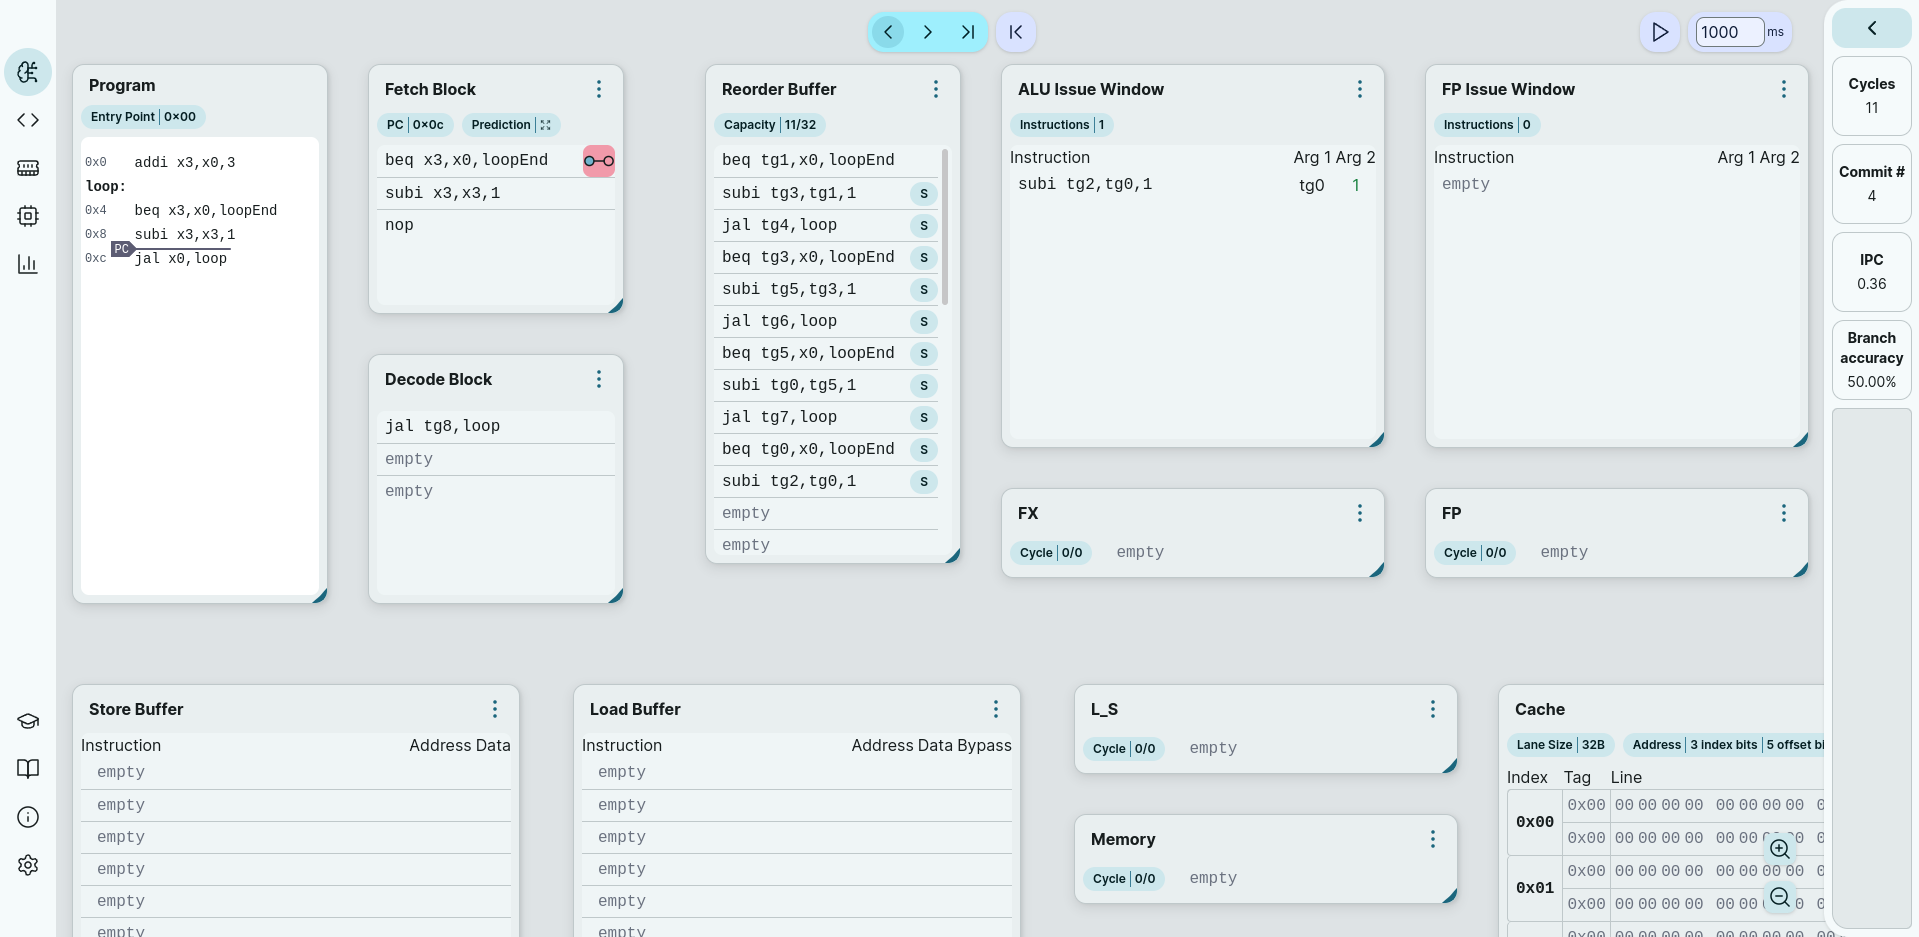
\includegraphics[width=\textwidth]{obrazky-figures/gallery/Selection_101.png}
    \captionof{figure}{caption}
    \label{fig:PropProf}
\end{minipage}}

\begin{sidewaysfigure}[ht]
    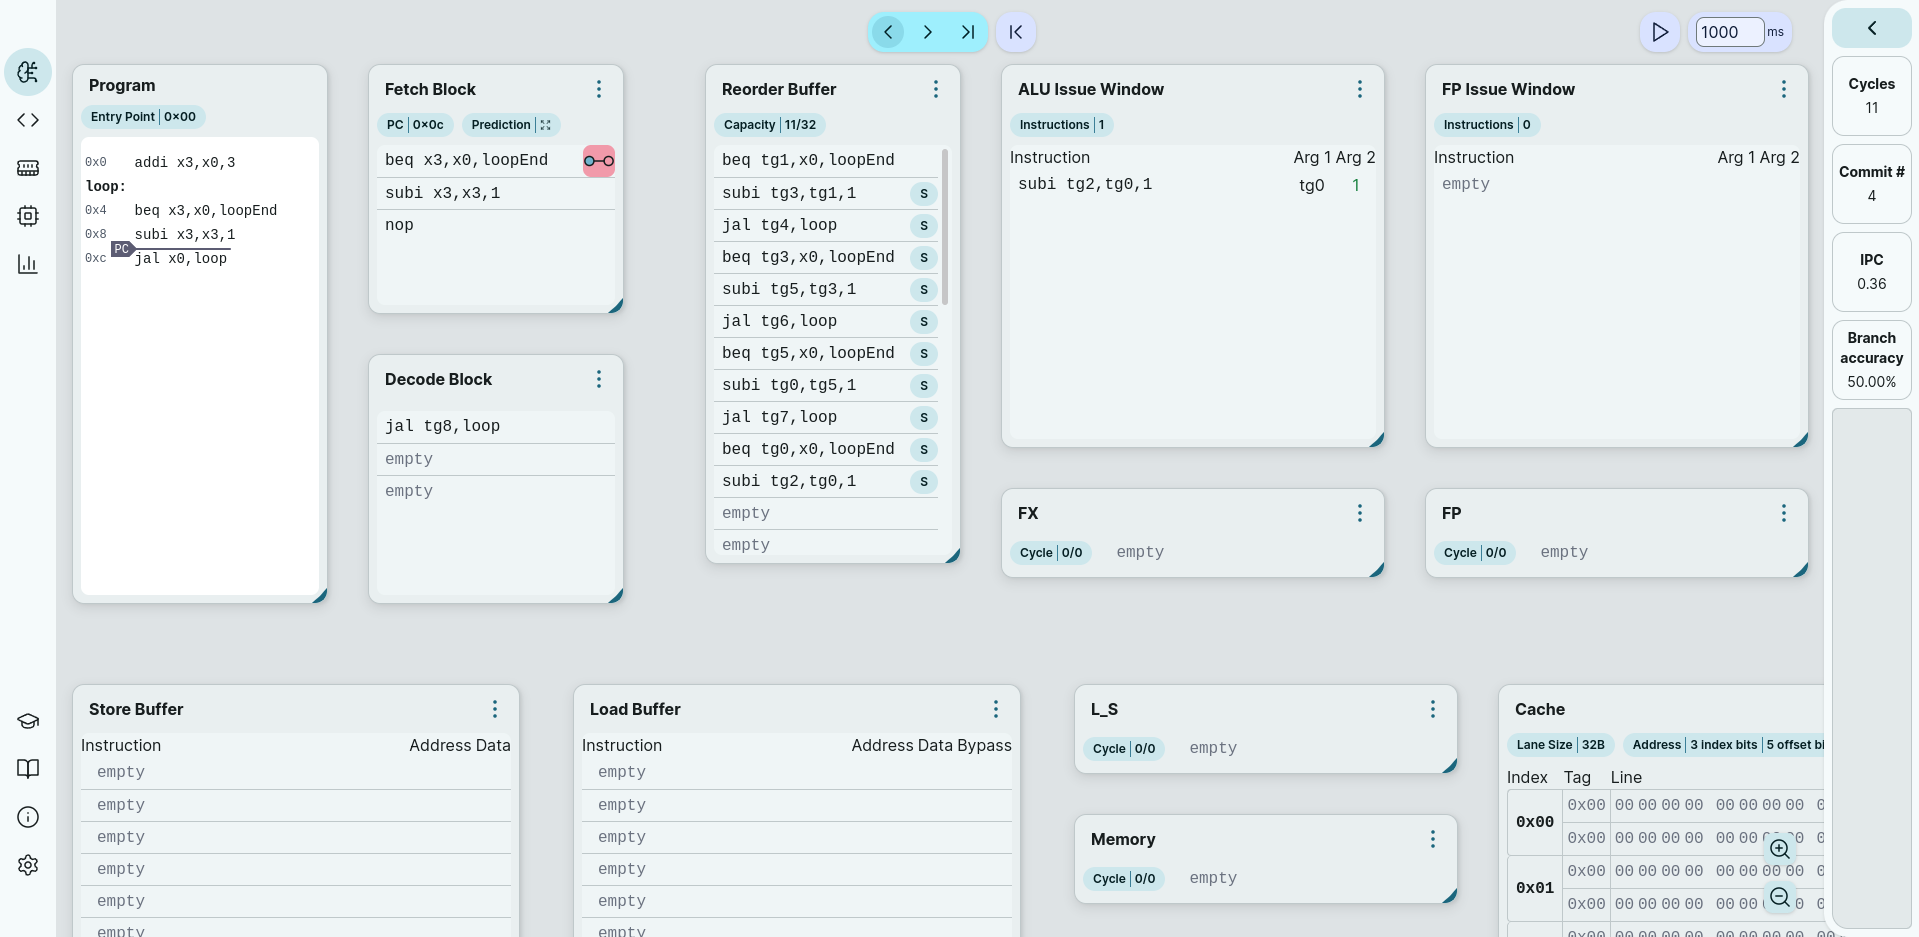
\includegraphics[width=\textwidth]{obrazky-figures/gallery/Selection_101.png}
    \caption{Hlavní okno aplikace -- procesor.}
    \label{gallery:main}
\end{sidewaysfigure}

\begin{sidewaysfigure}[ht]
    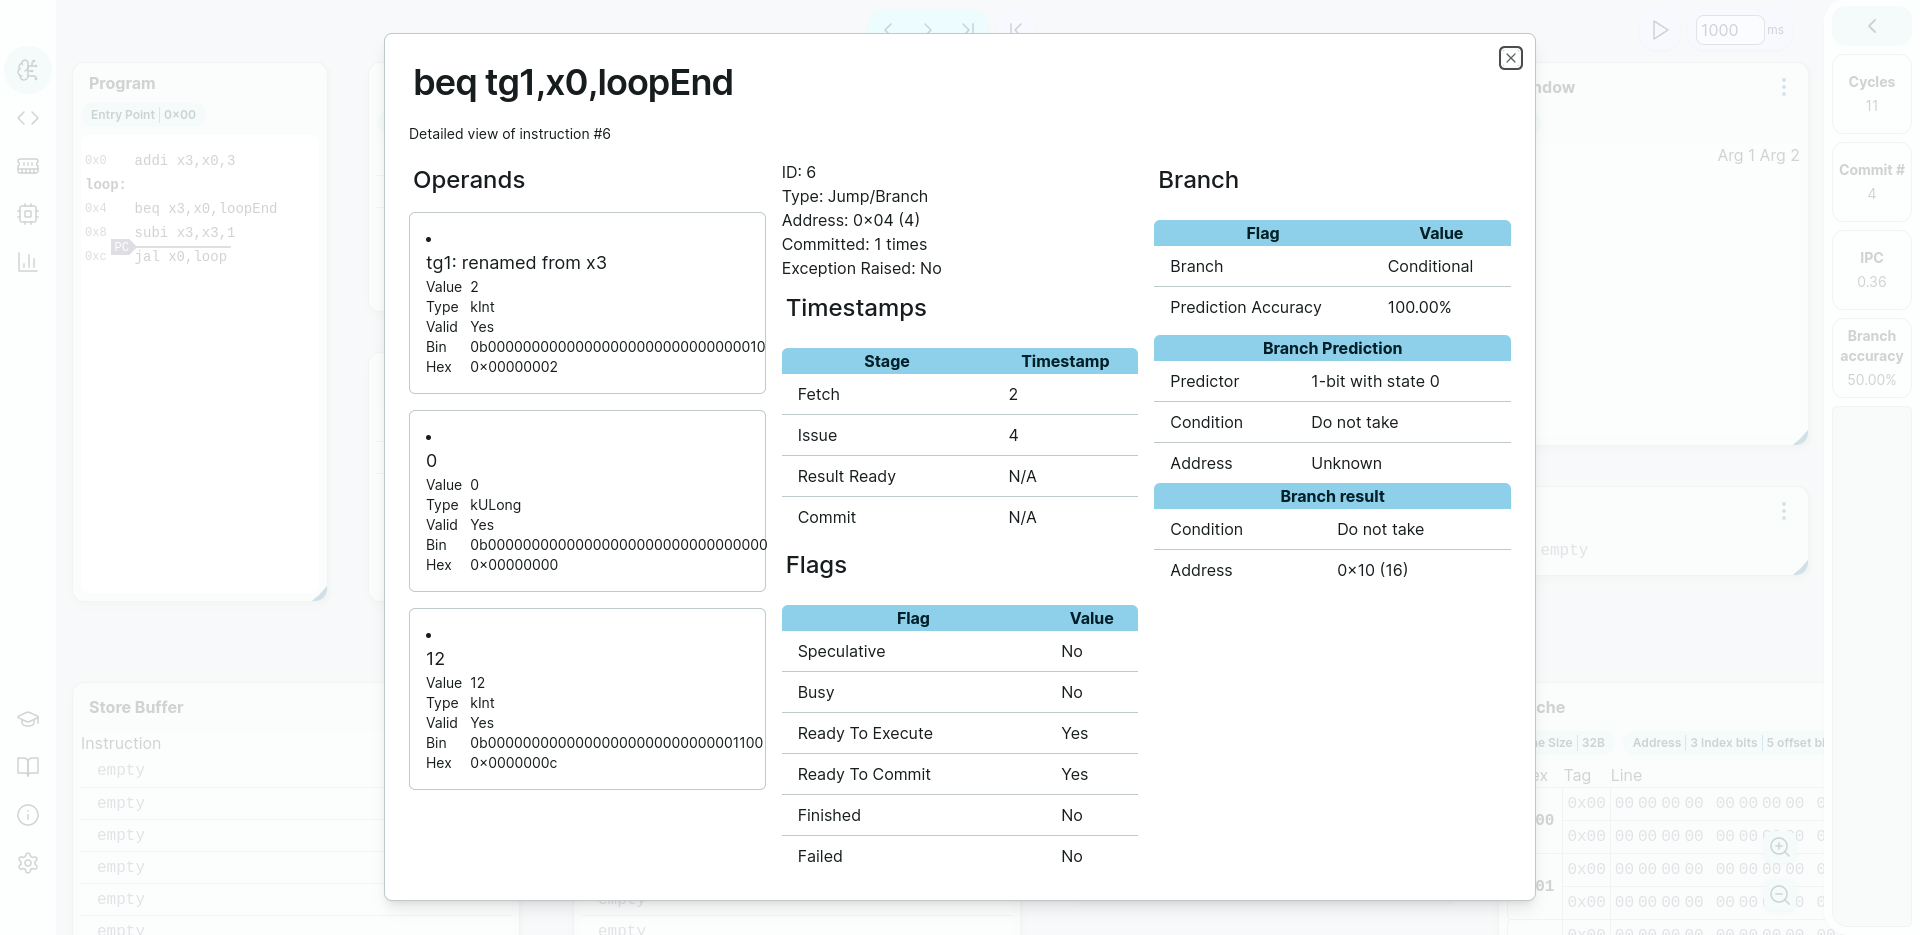
\includegraphics[width=\textwidth]{obrazky-figures/gallery/Selection_102.png}
    \caption{Detail konkrétní instrukce.}
    \label{gallery:instructionDetail}
\end{sidewaysfigure}

\begin{sidewaysfigure}[ht]
    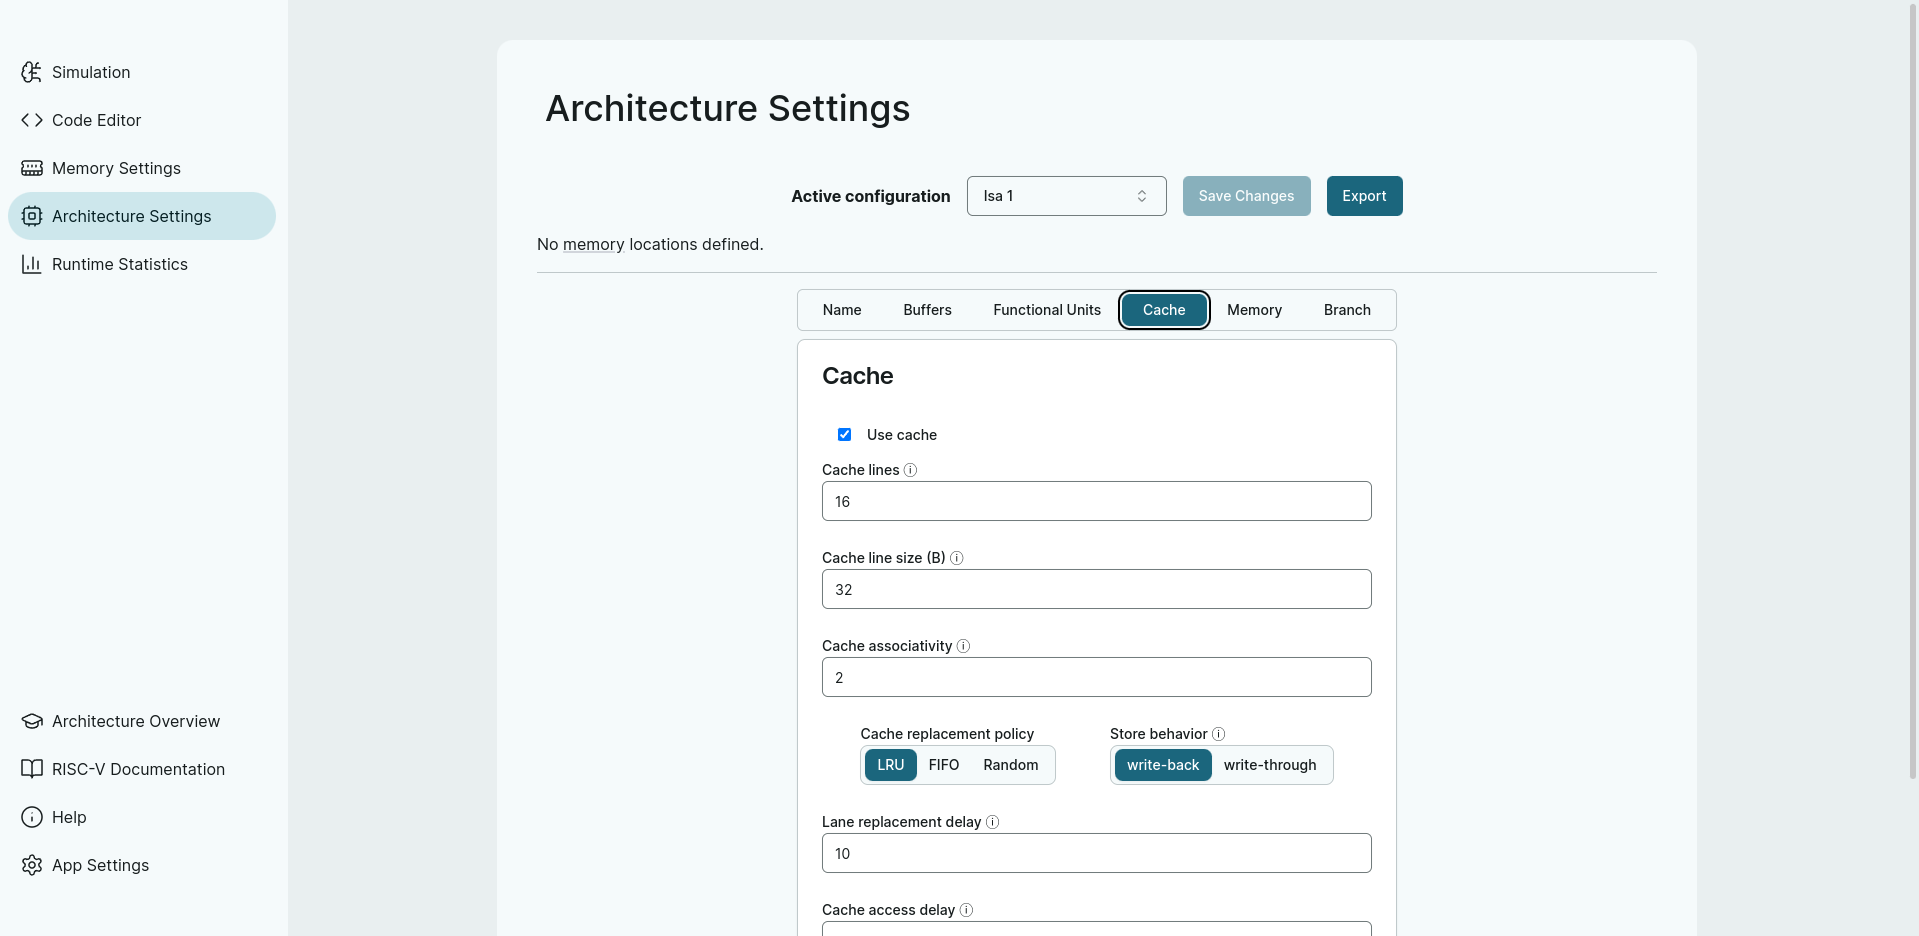
\includegraphics[width=\textwidth]{obrazky-figures/gallery/Selection_103.png}
    \caption{Konfigurační menu.}
    \label{gallery:isaconfig}
\end{sidewaysfigure}

\begin{sidewaysfigure}[ht]
    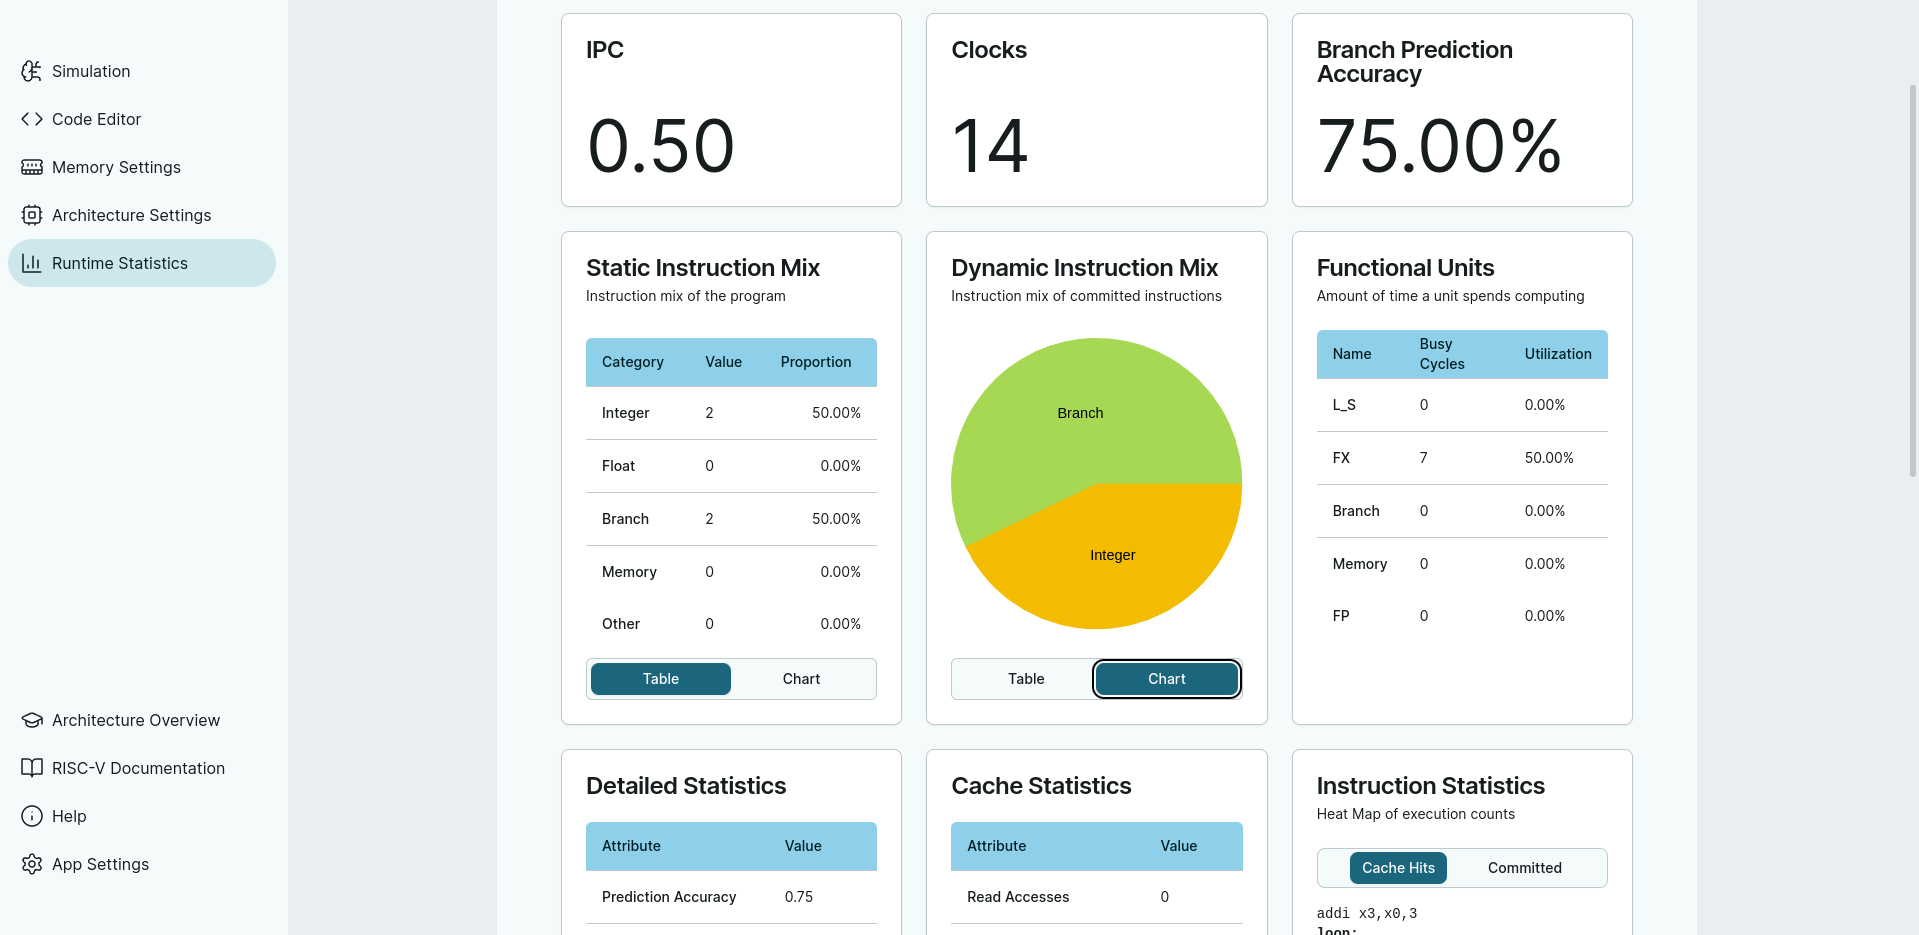
\includegraphics[width=\textwidth]{obrazky-figures/gallery/Selection_104.png}
    \caption{Běhové statistiky.}
    \label{gallery:stats}
\end{sidewaysfigure}

\begin{sidewaysfigure}[ht]
    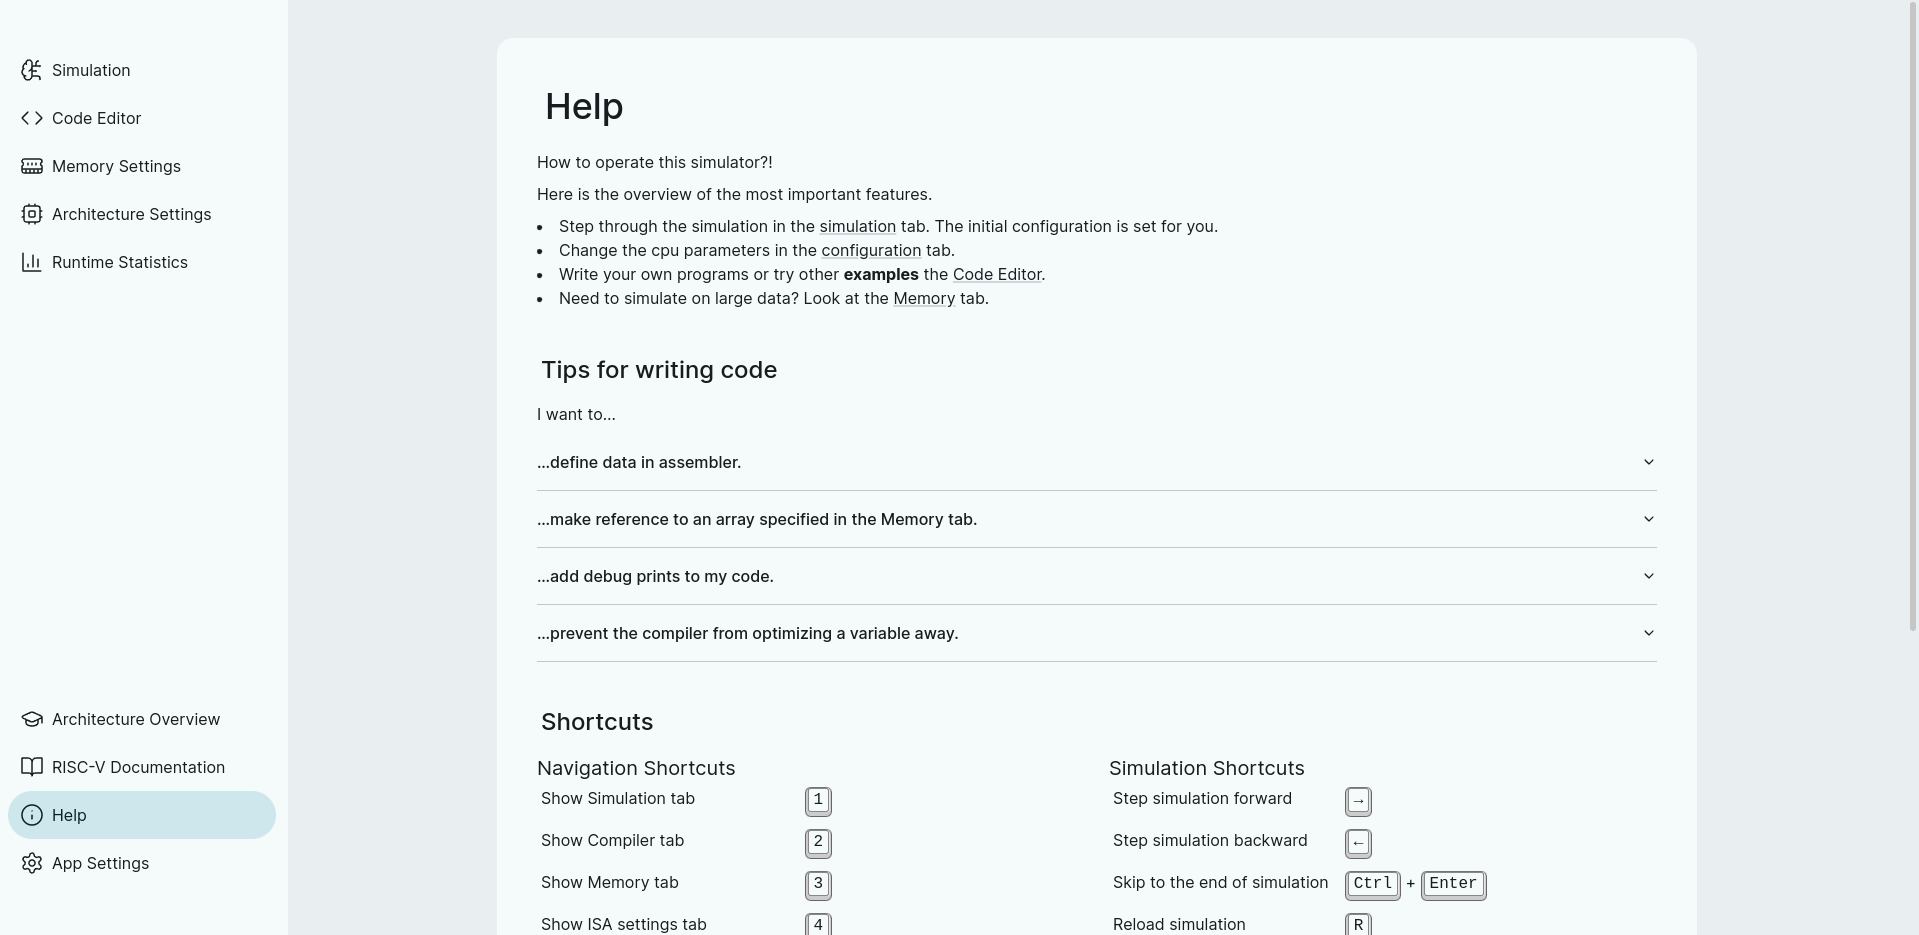
\includegraphics[width=\textwidth]{obrazky-figures/gallery/Selection_105.png}
    \caption{Návod k použití.}
    \label{gallery:help}
\end{sidewaysfigure}

\begin{sidewaysfigure}[ht]
    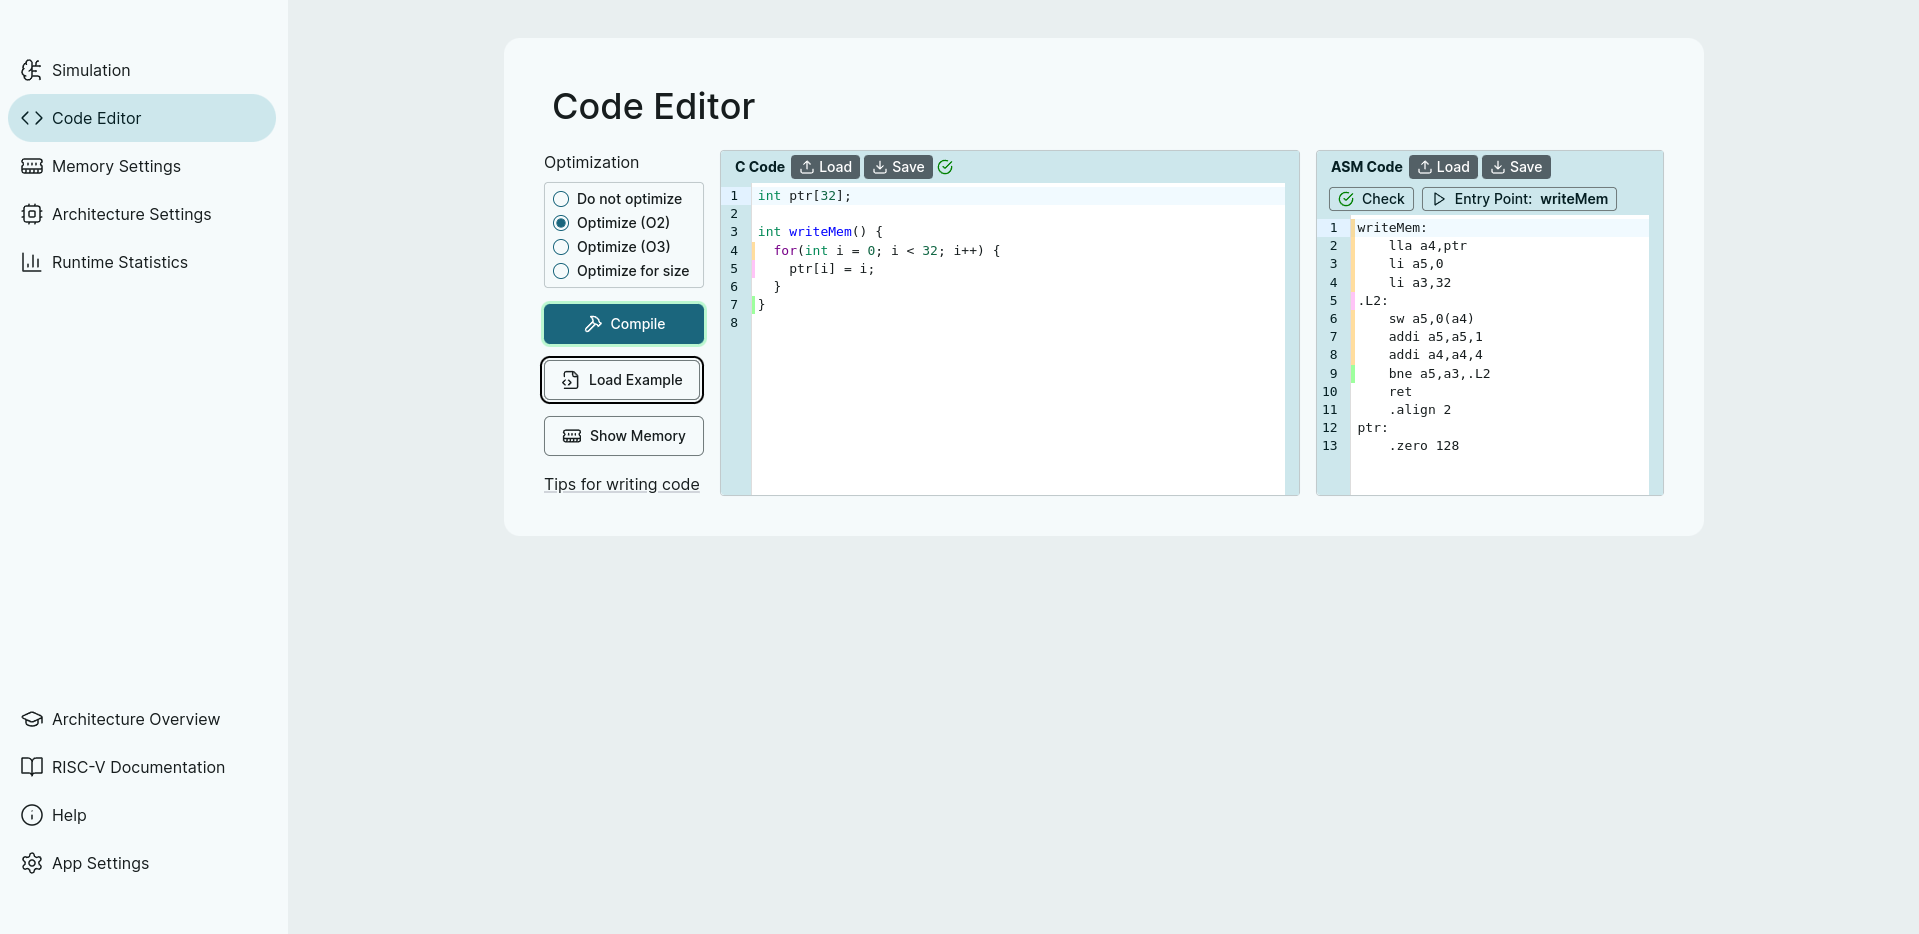
\includegraphics[width=\textwidth]{obrazky-figures/gallery/Selection_106.png}
    \caption{Editor kódu.}
    \label{gallery:compiler}
\end{sidewaysfigure}